%document information
\documentclass[10pt,a4paper]{book}

% packages
\usepackage[T2A]{fontenc}
\usepackage[utf8]{inputenc}
\usepackage[russian]{babel}

\usepackage{cmap} 
\usepackage{indentfirst} 
\usepackage{amsmath,amsthm,amssymb,amscd} 						
\usepackage[margin=2.3cm, footskip = 1 cm, headheight=36pt]{geometry}
\usepackage{emptypage}

\usepackage{epigraph}
\usepackage{tikz}
\usepackage{cancel}
															
\usepackage{xcolor}
\definecolor{darkblue}{rgb}{0,0,.6}
\definecolor{Purplemountainmajesty}{RGB}{150, 120, 182}

\usepackage{datetime}

\usepackage{lipsum}



\usepackage{graphicx}
\usepackage{caption}
\usepackage{microtype}

%РАБОТАЮЩИЙ ВЕЗДЕ В ТЕКСТЕ СЧЕТЧИК РИСУНОЧКОВ.
\newcounter{pictnumber}[chapter] 
\renewcommand{\thepictnumber}{\thechapter.\arabic{pictnumber}}

\input{insbox.tex}
\usepackage{threeparttable}

% IT WORKS EVERYWHERE EXCEPT LISTS! 
%it works in lists with \rightskip, but nevermind.

\newcommand*\addpicture[3][9]{\refstepcounter{pictnumber}%
\InsertBoxR{0}{\begin{threeparttable}\begin{tabular}{c@{}}\includegraphics[scale=#3]{#2}\end{tabular}\captionof{figure}{}\end{threeparttable}}[#1]}

% IT WORKS EVERYWHERE EXCEPT LISTS!
%it works in lists with \leftskip, but nevermind.

\newcommand*\addpicturel[3][9]{\refstepcounter{pictnumber}%
\InsertBoxL{0}{\begin{threeparttable}\begin{tabular}{c@{}}\includegraphics[scale=#3]{#2}\end{tabular}\captionof{figure}{}\end{threeparttable}}[#1]}

\usepackage{wrapfig}%for ez text
\newenvironment{mywrapfigure}
  {\refstepcounter{pictnumber}
	\begin{wrapfigure}}
  	{\end{wrapfigure}}


%SEE THE MOST POWERFUL CONSTRUCTION IN SUPERFILE.TEX
%IT IS THE NEXT CONSTRUCTION. but in superfile without "%"

% \begin{enumerate}
% \item 
%\refstepcounter{pictnumber}%  
%  \parbox[t]{\dimexpr\textwidth-\leftmargin}{%
%      \vspace{-2.5mm}
%      \begin{wrapfigure}{r}{0.5\textwidth}
%        \centering
%        \vspace{-2\baselineskip}
%        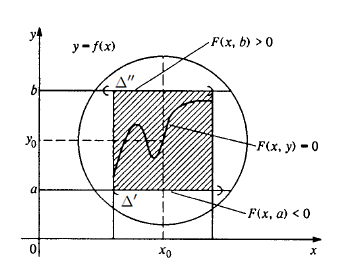
\includegraphics[scale=0.47]{ch9pict1.png}
%        \caption{}\label{kek}
%      \end{wrapfigure}
%         \lipsum[1]
%    }
%  \item     
%  \parbox[t]{\dimexpr\textwidth-\leftmargin}{%
%      \vspace{-2.5mm}
%      \begin{wrapfigure}[8]{r}{0.5\textwidth}
%      \end{wrapfigure}
%      \lipsum[2]
%}



\usepackage{titlesec, titletoc}
\titleformat{\chapter}[display]
  {\raggedright\normalfont\Large\bfseries}{\chaptertitlename\thechapter}{2ex}{}

\titleformat{\section}
  {\normalfont\Large\bfseries}{\thesection.}{1em}{}
\renewcommand{\thesection}{\textsection\arabic{section}}
\titlecontents{section}[2.7em]{\addvspace{0.5ex}}%
 {\contentslabel[\thecontentslabel.]{1.25em}\hskip0.8em}%numbered
 {}%numberless%
 {\enspace\titlerule*[0.7pc]{.}\contentspage}%

\renewcommand{\thesubsection}{\arabic{section}.\arabic{subsection}.}
  
\usepackage{fancyhdr}
\pagestyle{fancy}
\fancyfoot[C]{\thepage}
\fancyhead{}
\fancyhead [CE] {\nouppercase{\slshape \large \rightmark}}
\fancyhead [CO] {\nouppercase{\slshape \large \leftmark}}
\renewcommand{\chaptermark}[1]{%
 \markboth{\ifnum\value{secnumdepth}>-1 \chaptertitlename\thechapter \fi}{}%
}

\addto\captionsrussian{\renewcommand{\chaptername}{Билет №}}
   
% page settings 
\parindent=1cm
\binoppenalty=10000
\relpenalty=10000

% front page
\author{Андрей Диденко}
\title{Подготовка к ГОСу по МатАнализу \LaTeX
\thanks{Спасибо всем моим друзьям за поддержку в написании этого документа}
\date{16 Апреля 2016}}
  
% other settings
\pdfcompresslevel=9
\pdfobjcompresslevel=9

%own commands

\newtheoremstyle{note}%
{3pt}% Space above1
{3pt}% Space below1
{}% Body font
{}% Indent amount2
{\bfseries}% Theorem head font
{.}% Punctuation after theorem head
{.5em}% Space after theorem head3
{}% 

\theoremstyle{note}
\newtheorem{defn}{Определение}[chapter]
\renewcommand{\thedefn}{\arabic{defn}}
\newcommand{\theHdefn}{\thechapter.\arabic{defn}}

\newtheorem{defnn}{Определение} %штрихованное.
\renewcommand{\thedefnn}{\arabic{defn}'}
\newcommand{\theHdefnn}{\thechapter.\arabic{defnn}'}


\theoremstyle{plain}
\newtheorem{thm}{Теорема}[chapter]
\renewcommand{\thethm}{\arabic{thm}}
\newcommand{\theHthm}{\thechapter.\arabic{thm}}

\newtheorem{thmn}{Теорема}[chapter] %штрихованное.
\renewcommand{\thethmn}{\arabic{thm}'}
\newcommand{\theHthmn}{\thechapter.\arabic{thmn}'}


\newtheorem{cons}{Следствие}[chapter]
\renewcommand{\thecons}{\arabic{cons}}
\newcommand{\theHcons}{\thechapter.\arabic{cons}}

\newtheorem{consn}{Cледствие}[chapter] %штрихованное.
\renewcommand{\theconsn}{\arabic{cons}'}
\newcommand{\theHconsn}{\thechapter.\arabic{consn}'}


\newtheorem{lemm}{Лемма}[chapter]
\renewcommand{\thelemm}{\arabic{lemm}}
\newcommand{\theHlemm}{\thechapter.\arabic{lemm}}

\newtheorem{lemmn}{Лемма}[chapter] %штрихованное.
\renewcommand{\thelemmn}{\arabic{lemm}'}
\newcommand{\theHlemmn}{\thechapter.\arabic{lemmn}'}
  
\newtheorem{exmpl}{Пример}[chapter]
\renewcommand{\theexmpl}{\arabic{exmpl}}
\newcommand{\theHexmpl}{\thechapter.\arabic{exmpl}}

\newtheorem{stt}{Утверждение}[chapter]
\renewcommand{\thestt}{\arabic{stt}}
\newcommand{\theHstt}{\thechapter.\arabic{stt}}

\newtheorem{axiome}{Аксиома}[chapter]
\renewcommand{\theaxiome}{\arabic{axiome}}
\newcommand{\theHaxiome}{\thechapter.\arabic{axiome}}

\newtheorem{axiomen}{Аксиома}[chapter] %штрихованное.
\renewcommand{\theaxiomen}{\arabic{axiome}'}
\newcommand{\theHaxiomen}{\thechapter.\arabic{axiomen}'}


\numberwithin{equation}{chapter}
\renewcommand{\theequation}{\arabic{equation}}
\newcommand{\theHequation}{\thechapter.\arabic{equation}}

\newenvironment{solution}
  {\begin{proof}[Решение.]}
  {\end{proof}}

  

%special mention


\usepackage[breaklinks,pdftex,hyperindex,unicode]{hyperref}	
\hypersetup{
  pdftitle           = {GOS_MatAn},
  pdfauthor          = {Didenko Andre},
  pdfsubject         = {Matan},
  pdfstartview       = {FitH},
  pdfborder          = {0 0 0},
  bookmarksopen      = true,
  bookmarksnumbered  = true,
  bookmarksopenlevel = 2,
  colorlinks = true,     
  		linkcolor  = darkblue, 
  		urlcolor = Purplemountainmajesty
}